\documentclass[11pt,twocolumn]{article}
\usepackage[english]{babel}
\usepackage{amsmath,yhmath}
\usepackage{graphicx}
\usepackage[formats]{listings}
\usepackage[titletoc]{appendix}
\usepackage{color}
\usepackage[a4paper,top=0.8cm,left=0.8cm,right=0.8cm,bottom=1.5cm,marginparwidth=1.75cm]{geometry}
\usepackage{siunitx}
\usepackage[version=4]{mhchem}
\usepackage{csquotes}
\usepackage{hyperref}
\usepackage{url}
\usepackage{tabu}
\usepackage{subcaption}
\usepackage[compact]{titlesec}
\usepackage{multirow}
\usepackage{abstract}

\newcommand*{\rom}[1]{\uppercase\expandafter{\romannumeral#1}}
\allowdisplaybreaks
\lstdefineformat{C}{%
	\{=\newline\string\newline\indent,%
	\}=[;]\newline\noindent\string\newline,%
	\};=\newline\noindent\string\newline,%
	;=[\ ]\string\space}

\titlespacing\section{0pt}{12pt plus 4pt minus 2pt}{12pt plus 2pt minus 2pt}
\titlespacing\subsection{0pt}{12pt plus 4pt minus 2pt}{6pt plus 2pt minus 2pt}
\titlespacing\subsubsection{0pt}{12pt plus 4pt minus 2pt}{6pt plus 2pt minus 2pt}

\graphicspath{{figs/}}

\title{Internship report: stability test of 2008 COMPASS data }
\author{Yanzhao Wang\thanks{Email: yanzhao960808@gmail.com}\\
\textit{Bonn-Cologne Graduate School}\\
\textit{Rheinische Friedrich-Wilhelms Universit$\Ddot{a}$t Bonn}}
\date{October, 2019}

\begin{document}
\twocolumn[
  \begin{@twocolumnfalse}
    \maketitle
    \vspace{-0.8cm}
    \begin{abstract}
      The main goal of this project is to look for the abnormal runs from COMPASS experiment (2008). The COMPASS data being analyzed for each run were already preselected before the stability test. For seeking the abnormal runs, different parameters in each event are extracted and investigated, such as the position of primary vertices, angular distribution of recoiled protons, invariant mass of three pions, etc. By plotting values of the parameters from each different run, run number 70195, 69612, 70223, etc can be directly selected out because of disparities to the normal runs. The most significant abnormalities result from the inconsistency of half width value from pions and photons' invariant mass. The explanation of these disparities are made by further inspecting the corresponding photon number from ECAL2 and recoiled proton angular distribution.
\newline
\newline
\newline

    \end{abstract}
  \end{@twocolumnfalse}
  ]
\raggedbottom  
\saythanks
%Contents
\section{Introduction}
The COMPASS stands for "Common Muon and Proton Apparatus for Structure and Spectroscopy", a fixed target experiment for investigation of nucleon spin structure and hadron spectroscopy. The final experimental results are concluded by analyzing the data recorded by multiple detectors during scattering experiment. Due to the complexity and sensitivity of COMPASS detectors, recorded data can be easily sabotaged by unexpected external conditions, such as electronic malfunction or unusual shutdown of some components. The data with those unwanted effects should be selected out to improve the quality of data analysis in the final step. In this project, the abnormality resulting from these effects are only investigated for the data with different run numbers. By calculating and comparing values of multiple characteristic parameters of each run, the abnormal runs can be identified and further examined to postulate their probable causes. In the end, by checking the already existed information in log book, it then can be determined which runs should be discarded.
\section{Target and Detectors}
COMPASS experiment comprises large number of detectors, for identifying and measuring the particles coming out of interaction vertices. Additionally, there are also detectors which monitor the particle beams and trigger other components to decide when the signals should be read out or not. In this section, the basic functionalities of different kinds of detectors are introduced simply. 

\begin{figure*}[!ht]
	\centering
	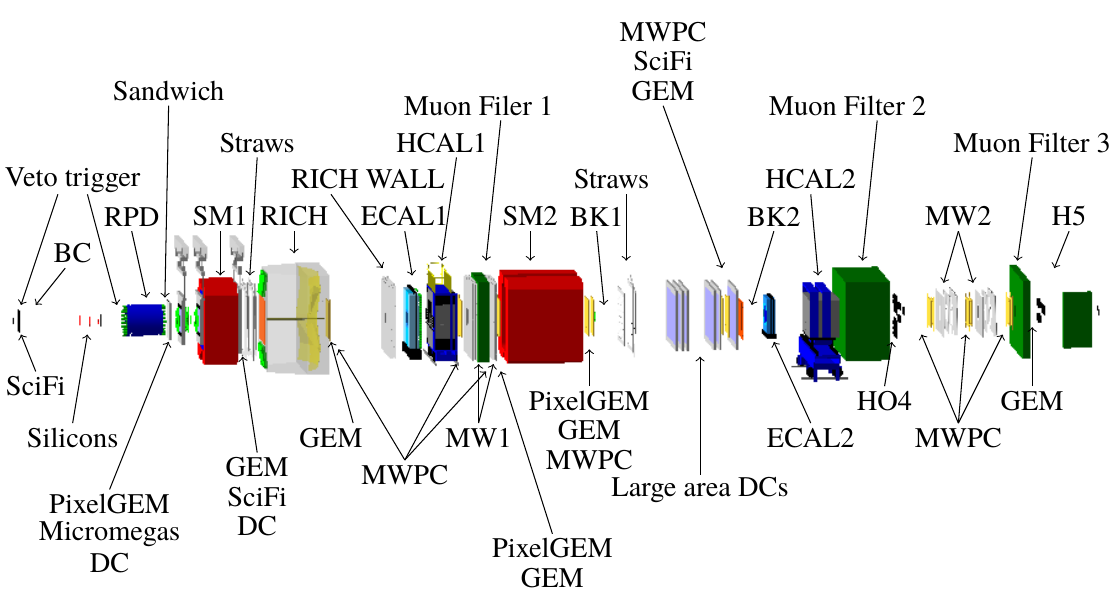
\includegraphics[width=\textwidth]{detector_layout}
	\caption{The layout of COMPASS detectors. The length of whole setup is around 50 meters. Pion beam comes from the left side of detectors and hits the target, which is surrounded by recoil-proton detector (RPD). On the right side of target, two different sets of detectors are used to measure out-going particles with small and large scattering angles.}
	\label{fig:detec_layout}	
\end{figure*}

\subsection{Particle beam and target}
To create the projectile particle beam, the proton beam, which is accelerated by the Super Proton Synchrotron (SPS), is firstly directed into Beryllium. From the nuclear reaction between proton and Beryllium nucleus, a secondary hadron particle beam is created, which functions as incoming particle beam for the scattering experiment. In this project, the hadron beam is selected to be negative charged pion beam. But a small fraction of Kaon (\SI{2.4}{\percent}) can also exist in the incoming particle beam. The proton target, onto which pion beam is diverted, is in form of liquid hydrogen stored in a \SI{40}{\centi\meter} height cylindrical container. 

\subsection{Detector layout}
\label{subsec:Detector_layout}
\begin{figure}[!th]
	\centering
	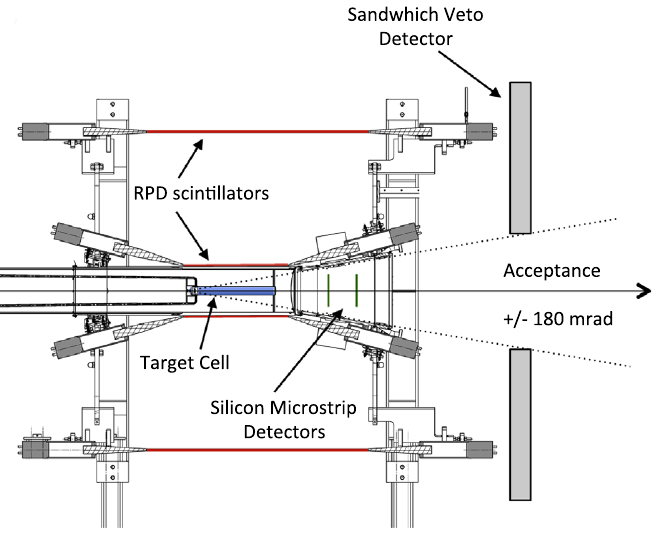
\includegraphics[width=0.5\textwidth]{sandwich}
	\caption{Scheme of detectors around the target region. The sandwich veto on the right prevent unmeasurable events with large scattering angles. Source: \cite{sandwich}}
	\label{fig:sandwich}
\end{figure}

The layout of COMPASS detectors is shown in figure \ref{fig:detec_layout}. Proton target is located inside the RPD (recoil-proton detector). On the left of target locate SciFi (scintillating fiber), BC (Beam counter) and silicon detectors. The coincidence of signals from SciFi and BC is used for the beam trigger, setting the time reference of whole system. The silicon detectors are applied for determining the location of projectile beam, which is further used to calculate the position of primary vertex. On the downstream very close to the target, there are sandwich veto and PixelGEM/Micromegas/DC (Pixel GEM detector, micromegas detectors and drift chamber). The function of sandwich veto is to reject the signal readout when the scattering polar angle of out-going particle is too large to measure. The structure of sandwich veto can be seen in figure \ref{fig:sandwich}, where the veto can be triggered if polar angle is out of acceptance range. Behind the sandwich veto, PixelGEM/Micromegas/DC detectors are implemented to measure the angles of out-going particles with high accuracy and resolution. On the downstream further away from the target, two different sets of detectors are set up for measuring out-going particles with small and large scattering angles. 

The first set, located in the front, is used as large angle spectrometer (LAS). The major components of LAS are SM1 (solenoid magnet 1), tracking detectors, RICH (ring-image Cherenkov detector), ECAL1, HCAL1 and Muon filter. SM1 provides the magnetic field to deviate charged particles. The degree of deviation is measured by the tracking detectors on the both sides, which can calculate the momentum of out-going charged particles. The RICH detector on the right side on SM1 is used to improve the permanence of experiment by separating $\pi$ and $K$ in high intensity environment\cite{RICH}. ECAL1 is an electromagnetic calorimeter used to measure the energy of particles like electrons or photons while HCAL1, a hadron calorimeter, is used to measure the energy of hadron particles. Muon can be identified by tracking detectors behind a muon filter, which intercepts every particles except muon.

The second set, located at the end of downstream, is deployed as small angle spectrometer (SAS). Most of its components have the same functionalities as their counterparts in LAS. The main additional detectors in SAS contains two BKs (beam killer), which are basically two scintillating counters. They are used to veto the non-interacting particle beams\cite{sandwich}.







\section{Data and interaction}
The data recorded by multiple detectors are stored in different partitions. Before carrying out the stability test in this project, the data being analyzed are already pre-selected. In this section, an overview about data storage and pre-selection is discussed, followed by a short introduction of probable interaction giving rise to selected data.

\begin{figure}[t!]
	\centering
	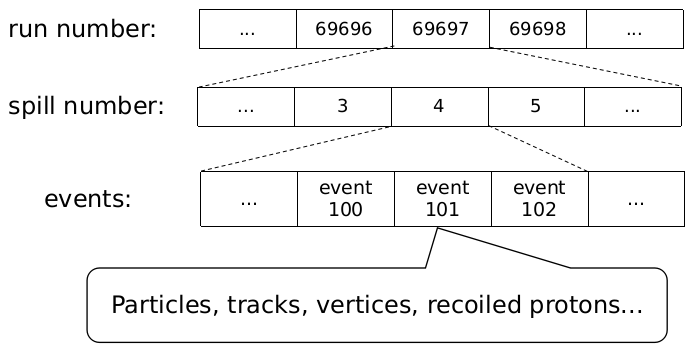
\includegraphics[width=0.5\textwidth]{data_storage}
	\caption{Scheme of data storage structure. Data from the detectors are categorized into three different levels.}
	\label{fig:data_storage}
\end{figure}

\subsection{Data storage}
There are three different partition levels regarding the data storage, as is shown in picture \ref{fig:data_storage}. First, the whole data are stored with different run number. The event data with same run number are further divided into different spill number. One spill corresponds to one period of process, in which the particle beam is bunched and de-bunched. Time expansion of each spill is around 48 seconds \cite{COMPASS}, which is time period of SPS (super proton synchrotron). Similarly, each spill contains large amount of events. One event represents a single scattering between $\pi$ and proton and it contains all data of the corresponding event from detectors such as tracking detectors or calorimeters.

\subsection{Data preselection}
\label{subsec:data_preselection}
The data used in this stability test are not raw data coming directly from detectors, but rather being preselected previously. Event is only selected if it meets following 4 conditions: 
\begin{itemize}
	\item A best primary vertex was found
	\item Primary vertex Z-position $Z_{pv}$: $\SI{-200}{\centi\meter} < Z_{pv} < \SI{160}{\centi\meter}$
	\item Exactly one or three charged tracks, leaving the primary vertex
	\item Charge sum of all three tracks $= -1$
\end{itemize}
The first condition requires the existence of primary vertex. This is because the vertex position is not the value that can be directly measured by detectors. It is rather reconstructed by identifying the intersecting point between two charged particle tracks. Thus, there could be no primary vertex constructed in some events, which should be selected out. Second condition excludes the events where outgoing particles are not coming from the interaction on proton target but rather on some detectors. Therefore, the position of primary vertex must be around the target region. The third and fourth condition guarantees the data after selection correspond to the elastic scattering or the interaction where one $\pi$ is scattered into three charged $\pi$.

\subsection{Scattering process}
\label{subsec:photon}
\begin{figure}[thb]
	\centering
	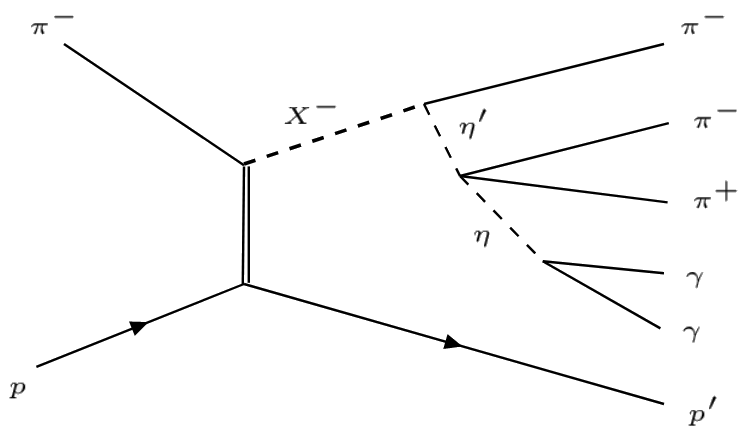
\includegraphics[width=0.5\textwidth]{feymann_diag}
	\caption{Scheme of one possible inelastic scattering between $\pi$ and proton. In such case, $pi^-$ is excited and consecutively decays into 3 charged $\pi$, during which multiple photons can also be emitted.}
	\label{fig:feymann_diag}
\end{figure}

The interaction that is looked into for this stability test is inelastic scattering of one $\pi^-$ scattered into three charged $\pi$. Due to the preselection, charged ejectile particles are very likely to be $\pi^-$, $\pi^+$, $\pi^-$.  One possibility of the interaction is shown in figure \ref{fig:feymann_diag}. By scattering off the proton target, $\pi^-$ is excited into a high energy state ($X$), which in a very short time, decays into $\pi^-$ and $\eta'$. Due to instability of $\eta'$, it finally decays into $\pi^-$ and $\pi^+$ as well. Meanwhile, certain number of photons can also be emitted by electromagnetic radiation. 
\section{Analysis and results}
\section{Conclusion}
In this project, to analysis the instability of different runs from COMPASS experiment, different parameters are extracted or calculated for each run. Among characteristic parameters such as the total number of events or invariant mass of three pions, the total invariant mass of out-going particles prove to be the most indicative parameters. Its correlation with ECAL1 photon number percentage ($\alpha$) encompasses most of abnormal runs found during stability test. The positive correlated regions also indicate the abnormality in angular distribution of recoil proton whereas negative correlated regions are related to the decline of ECAL2 averaged photon number per event. By checking out the logbook of experiment, some abnormality could be well explained such as the malfunctions of sandwich veto or solenoid magnet.

% BIBLIOGRAPHY
\bibliographystyle{plain}
\clearpage
\bibliography{references}

%Appendix
%\cleardoublepage

%\input{chapters/Appendix}
\end{document}


